\chapter{Materiais e Métodos}
\label{cap:materiais-metodos}

Nesta seção, detalha-se o enquadramento metodológico construído para
responder à questão central desta pesquisa: \emph{como a análise de
sentimento por aspecto, apoiada por Modelos de Linguagem de Grande Porte e
dados perceptivos georreferenciados, pode auxiliar a identificar gargalos
no desempenho de ODS municipais e gerar diagnósticos acionáveis para
políticas públicas?} Os conceitos teóricos que sustentam esta abordagem ---
incluindo a arquitetura Transformer, o modelo \gls{BERT}, os \gls{LLM}s
generativos e as técnicas de análise de sentimentos --- foram apresentados
no Capítulo~\ref{cap:fundamentacao-teorica}. Este capítulo concentra-se,
portanto, nas escolhas e procedimentos metodológicos, na seleção e
comparação das ferramentas de análise e nos resultados parciais obtidos
durante a fase de prototipação.

A modalidade metodológica adotada neste trabalho é a Design Science,
conforme definido por \citeauthor{wieringa2014} \citeyear{wieringa2014} e
detalhada no Capítulo~\ref{cap:introducao}. Esta escolha alinha-se aos
objetivos de desenvolver e avaliar um artefato tecnológico --- um sistema
automatizado de análise de ODS municipais --- e, simultaneamente, gerar
conhecimento sobre como técnicas de \gls{NLP} e \gls{LLM}s podem auxiliar
no diagnóstico de gargalos de desempenho em escala local. As etapas da
Design Science, envolvendo a construção do artefato, sua aplicação em
estudos de caso reais e a avaliação por especialistas, guiam a pesquisa. A
análise de sentimento por aspecto, aplicada a avaliações públicas
georreferenciadas coletadas via Google Places API, é o principal mecanismo
investigativo, permitindo a identificação sistemática de padrões e
problemas associados a estabelecimentos físicos concretos.

\section{Análise de Ferramentas}
\label{sec:analise-ferramentas}

A seleção de uma ferramenta ou abordagem para análise de sentimento
envolve considerar um espectro de opções, cada uma com suas características,
vantagens e desvantagens. Conforme detalhado no
Capítulo~\ref{cap:fundamentacao-teorica}, as abordagens disponíveis vão
desde métodos baseados em léxicos até modelos neurais profundos baseados em
Transformers e LLMs generativos.

Abordagens mais simples, como as baseadas em léxicos de polaridade e regras heurísticas --
a exemplo da biblioteca TextBlob, que oferece uma interface simplificada para tarefas de NLP,
incluindo análise de sentimento em Python \cite{loria2018}, e do modelo VADER (\textit{Valence Aware
Dictionary and sEntiment Reasoner}), especificamente desenvolvido e validado para a análise de
sentimento em textos de mídias sociais \cite{hutto2014} -- são fáceis de implementar e oferecem
resultados rápidos. O VADER, em particular, é otimizado para dados de mídias sociais. No entanto,
essas abordagens podem apresentar baixa precisão em textos com contextos complexos, ironia ou
gírias. Bibliotecas como NLTK também oferecem funcionalidades para análise de sentimentos,
muitas vezes combinando léxicos com aprendizado de máquina, mas podem requerer maior
configuração \cite{bird2009}.

O aprendizado de máquina tradicional, como o utilizado pelo FastText \cite{joulin2017},
que emprega \textit{word embeddings} e modelos lineares como a regressão logística para classificação de
texto, oferece maior eficiência e escalabilidade para grandes volumes de dados, mas geralmente
necessita de treinamento em volumes consideráveis de dados para alcançar bons resultados.

Modelos baseados em Transformers, como o BERT e suas variantes (RoBERTa, BERTimbau),
representam o estado da arte em termos de precisão para análise de sentimento contextual.
Plataformas como Hugging Face, através da biblioteca \textit{transformers} \cite{wolf2020}, facilitam o
acesso a esses modelos pré-treinados, que podem ser adaptados (\textit{fine-tuned}) para tarefas
específicas. Contudo, o \textit{fine-tuning} e a inferência com esses modelos podem ser
computacionalmente intensivos.

Paralelamente, existem serviços de NLP em nuvem, como o Google Cloud Natural Language
\gls{API} \cite{googlecloud2025} e o Azure Text Analytics, atualmente integrado ao Azure AI Language
\cite{microsoftazure2025}. Estes serviços oferecem APIs de fácil integração para análise de
sentimento e outras tarefas de NLP, sem a necessidade de gerenciamento de infraestrutura ou
treinamento de modelos por parte do usuário, embora geralmente impliquem custos e menor
controle sobre o modelo subjacente. Essas comparações podem ser vistas na Figura
\ref{tab:comparativa-ferramentas}.

\begin{figure}[h]
    \centering
    \caption{Tabela Comparativa das Ferramentas}
    \label{tab:comparativa-ferramentas}
    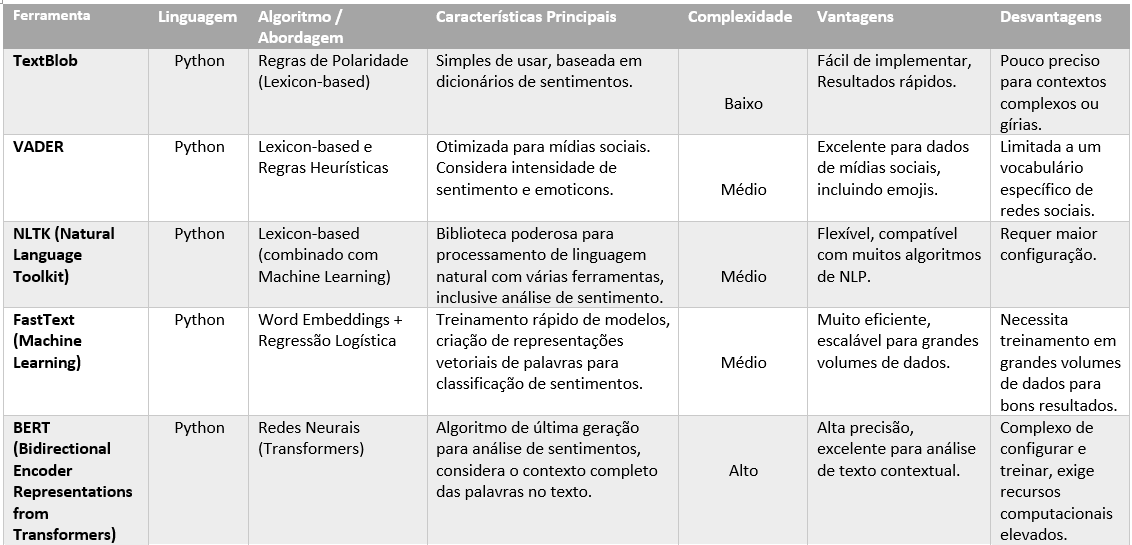
\includegraphics[width=\textwidth]{figuras/tabela-comparativa-ferramentas}
    \legend{Fonte: Autoria Própria (2025).}
\end{figure}

\section{Resultados Parciais}
\label{sec:resultados-parciais}

A análise das implementações desenvolvidas demonstrou que alguns modelos podem se sobressair a outros conforme veremos a seguir. Esta superioridade
manifesta-se através de diversas características técnicas que evidenciam tanto a eficiência quanto a
qualidade dos resultados obtidos.

A implementação com Gemini destaca-se inicialmente por sua simplicidade, como pode ser
visto na Figura \ref{fig:eficiencia-codigo}. Enquanto as implementações utilizando OpenAI e Cohere
requereram 146 linhas de código cada uma, a solução com Gemini é significativamente mais
concisa, utilizando apenas 89 linhas. Esta diferença não representa apenas uma economia de código,
mas reflete uma arquitetura mais elegante e menos propensa a falhas. Diferentemente das outras
APIs que necessitam de sistemas complexos de \textit{retry} -- ou seja, mecanismos que automaticamente
tentam enviar uma nova requisição em caso de falha -- para lidar com erros temporários, o Gemini
demonstrou maior estabilidade durante os testes, não apresentando falhas de processamento.

\begin{figure}[h]
    \centering
    \caption{Eficiência do Código}
    \label{fig:eficiencia-codigo}
    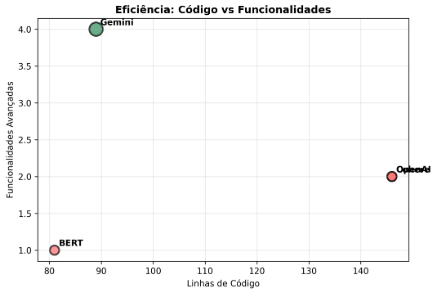
\includegraphics[width=0.85\textwidth]{figuras/eficiencia-codigo}
    \legend{Fonte: Autoria Própria (2025).}
\end{figure}

A capacidade de resposta estruturada do Gemini constitui outra vantagem significativa. O
modelo fornece não apenas a classificação do sentimento, mas também um valor de confiança
numérico e justificativas detalhadas para cada análise. Esta funcionalidade permite uma avaliação
mais precisa da qualidade dos resultados e facilita a interpretação dos dados por parte dos
pesquisadores. As justificativas geradas pelo Gemini demonstraram ser consistentemente mais
elaboradas e contextualmente relevantes conforme pode ser visto na Figura \ref{fig:nivel-confianca},
considerando tanto o conteúdo textual quanto as avaliações numéricas associadas aos \textit{reviews} de testes utilizados nas análises.

\begin{figure}[h]
    \centering
    \caption{Nível de Confiança}
    \label{fig:nivel-confianca}
    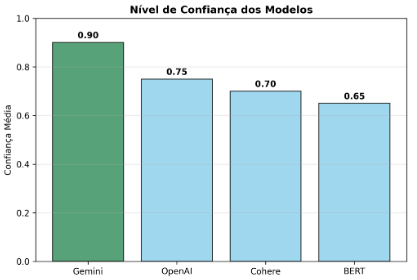
\includegraphics[width=0.85\textwidth]{figuras/nivel-confianca}
    \legend{Fonte: Autoria Própria (2025).}
\end{figure}

Em contraste, as limitações das outras implementações tornaram-se evidentes na comparação
conforme pode ser analisado na Figura \ref{fig:taxa-erro}. A solução OpenAI, embora robusta,
requer configurações mais verbosas com \textit{roles} de sistema, ou seja, instruções que definem como a
IA deve se comportar e responder, e demonstrou maior propensão a falhas temporárias durante os
testes. O sistema de \textit{retry} que foi preciso ser implementado, apesar de necessário para garantir
estabilidade, adiciona complexidade desnecessária ao código e pode impactar a velocidade de
processamento. Já a implementação com BERT multilingual, embora processe dados localmente, o
modelo que foi utilizado para teste apresentou limitações significativas como a restrição de 512
\textit{tokens} por texto e a dependência de classificações baseadas em estrelas, que se mostraram menos
interpretáveis para análises qualitativas.

\begin{figure}[h]
    \centering
    \caption{Taxa de Erro dos Modelos}
    \label{fig:taxa-erro}
    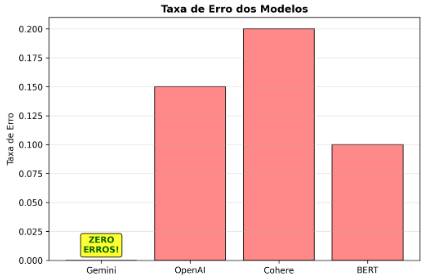
\includegraphics[width=0.85\textwidth]{figuras/taxa-erro}
    \legend{Fonte: Autoria Própria (2025).}
\end{figure}

Os resultados obtidos demostram uma possível superioridade do Gemini. A análise dos dados
processados revela que o modelo mantém uma confiança média consistente entre 0,8 e 0,95,
indicando alta precisão nas classificações. Mais importante ainda, durante todos os testes
executados, o Gemini não apresentou erros de processamento, demonstrando uma confiabilidade
operacional superior às demais soluções como pode ser visto na Figura \ref{fig:performance}. As
justificativas geradas pelo modelo mostram-se particularmente sofisticadas, considerando nuances
contextuais que outros modelos frequentemente ignoram.

\begin{figure}[h]
    \centering
    \caption{\textit{Performance}}
    \label{fig:performance}
    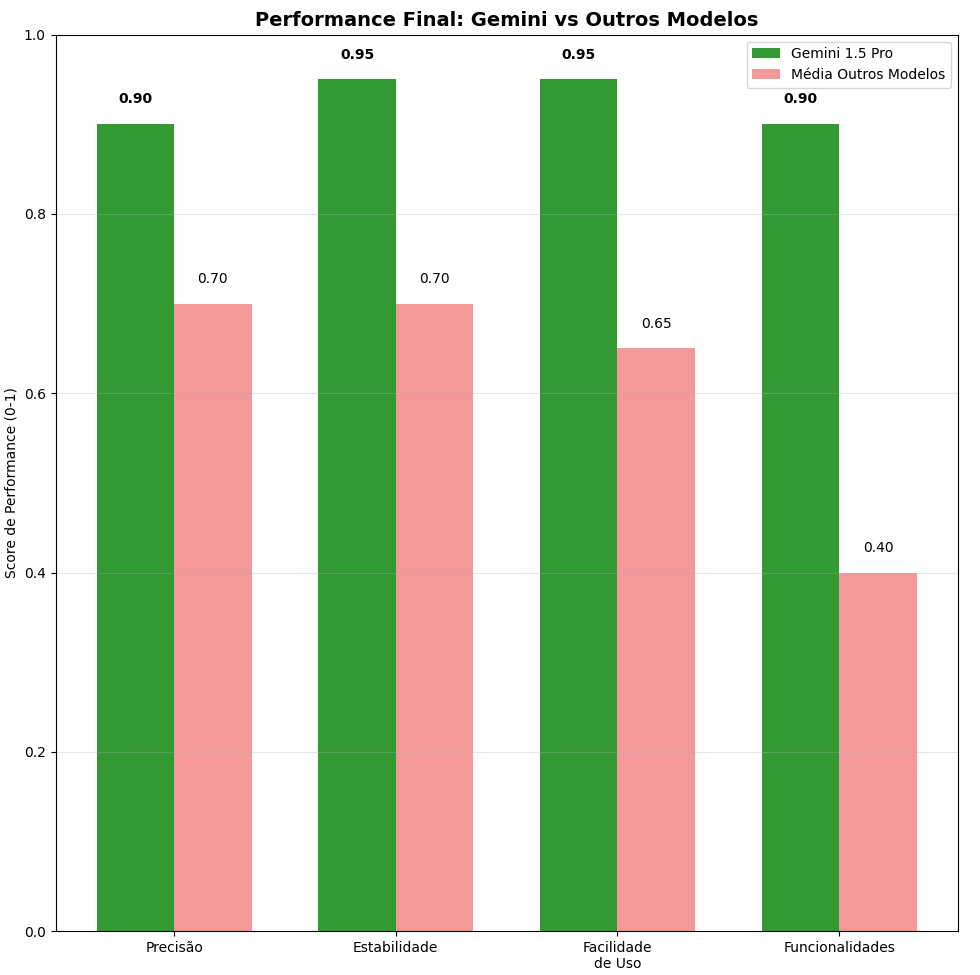
\includegraphics[width=0.85\textwidth]{figuras/performance}
    \legend{Fonte: Autoria Própria (2025).}
\end{figure}

Um exemplo representativo desta qualidade pode ser observado em uma análise onde o
Gemini identificou corretamente um sentimento positivo com confiança de 0,95, justificando que o
usuário descrevia o lugar como ótimo e sugeria atividades agradáveis para família e amigos,
reforçando esta interpretação com a avaliação numérica de 5 pontos. Esta capacidade de síntese
entre elementos textuais e numéricos demonstra uma compreensão contextual superior que se
traduz em resultados mais precisos e úteis para pesquisas acadêmicas.

Dessa forma, os resultados parciais estabelecem claramente que a implementação com
Google Gemini Pro constitui a solução mais promissora para análise de sentimentos em
\textit{reviews} com foco em sustentabilidade. A combinação de robustez técnica, capacidade analítica
superior, flexibilidade contextual e qualidade excepcional das respostas posiciona esta
implementação como ferramenta essencial para pesquisas em turismo sustentável e práticas ESG,
oferecendo não apenas maior precisão técnica, mas também funcionalidades avançadas que abrem
novas possibilidades de análise em estudos sobre percepções de sustentabilidade no setor turístico.
